
\section{Background}

We assume a background on LLMs, including their transformer-based architecture (\Cref{app:llm-transformer}), in-context learning (\Cref{sec:icl-performance}), and reinforcement learning (full preliminaries are provided in \Cref{app:technicality}). We briefly review the literature on mnemonic devices for vocabulary learning and the use of LLMs in linguistic tasks.

\subsection{Mnemonic devices for vocabulary learning}

\begin{table*}[htb]
\centering
\caption{Examples of feature categories for English words.}
\label{tab:linguistic-features}
\begin{tabularx}{\textwidth}{l >{\raggedright\arraybackslash}X >{\raggedright\arraybackslash}X}
\toprule
\textbf{feature} & \textbf{description} & \textbf{example} \\
\midrule
\textbf{phonetics} & vocab's sound patterns & \emph{apparent} sounds like “a bare Asian.” \\
\addlinespace
\textbf{orthography} & written/spelling patterns & \emph{abet} looks like “a + bet.” \\
\addlinespace
\textbf{morphology} & structure including free and bound morphemes & \emph{aggrandize} = a + grand + –ize, to mean to make grander. \\
\addlinespace
\textbf{etymology} & vocab origin and history & \emph{adumbrate} comes from Latin ad- (to, on) + umbra (shade) + ate, to mean foreshadow or outline. \\
\addlinespace
\textbf{semantics} & vocab meaning and relationships & \emph{confound} has similar meaning and history with 'confuse'. \\
\bottomrule
\end{tabularx}
\end{table*}

% TODO: Add a figure for what good mnemonics means. Here is a placeholder
\begin{figure}
  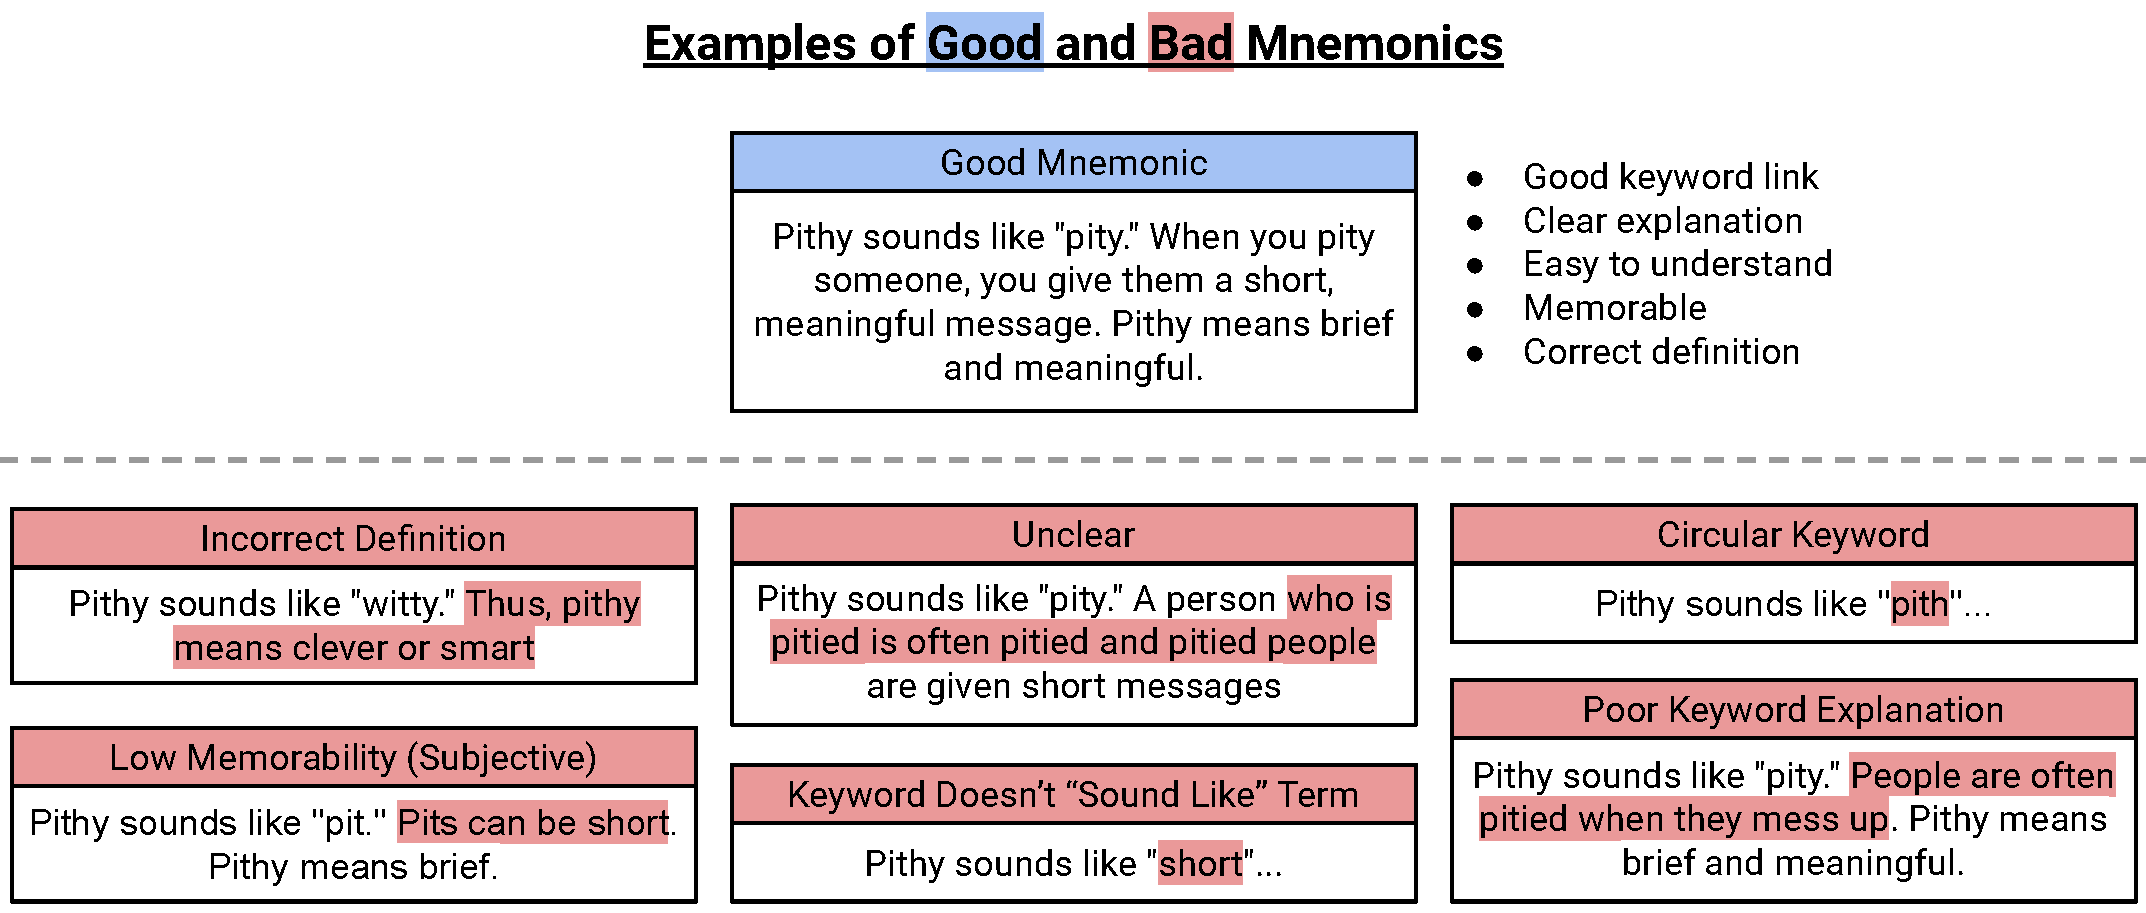
\includegraphics[width=\linewidth]{figures/good_bad_mnemonics.pdf}
  \caption{Non-exhausitive list of characteristics of a good mnemonic, inferred from \citetext{\citealp{BalepurSMART2024}, \citealp{CamposUSING2011}, \citealp{SariogluUSE2024}}.}
  \label{fig:good-mnemonic}
\end{figure}
\subsection{LLMs: linguistic competence and creativity}
